\chapter{图上函数的变换与查询}
\label{chap:graph-functions}

同一张四顶点图上可以放三类很不一样的计算。给每个顶点记一个温度，得到四个可相加的实数，
任务是让相邻点的取值不要差得太悬殊；给每个顶点一个类别，得到只能比较同异的离散标记，
任务是描述它周围有哪几类邻居、各有几个；给四个二值变量一次完整赋值，
则要面对$2^4=16$种配置，任务是求总权重、最优配置或保留部分变量后的一张表。
连接结构相同，允许的运算和输出却不同，不能因为都“沿边传消息”就把它们当成一回事。

本章先在5.1节区分这三类函数对象与它们的输入输出；5.2节把顶点数值变换成由本图拉普拉斯决定的
模态坐标（图傅里叶）；5.3节按给定的频率响应处理顶点信号，包括多项式局部滤波、连续热扩散
和它的显式时间离散；5.4节处理离散标记的邻域细化；5.5节处理配置函数，
说明在什么运算规则下可以消去内部变量、怎样在树和树分解上复用接口表。
最后一节离开固定的图，在子集格上讨论由累计值恢复各子集自身贡献的Möbius反演。
这些方法都不学习参数；具体图网络的函数族、训练与表达能力留待神经网络卷。
本章固定含$n\geq1$个顶点的有限无向非负权图，结构邻接与正权支撑沿用第~\ref{chap:graph-objects}章约定。

\section{图上函数计算的基本概念}

\paragraph{顶点数值与\term{图信号}}
给每个顶点一个实数得到$f:V\to\mathbb R$，固定顶点次序后只需存$n$个实数，称图信号。
对它做邻居加权平均会改变数值，做谱投影则改变表示而不改变信号本身——前者是处理，后者是换坐标。

\paragraph{离散顶点标记}
给每点一个类别得到$c:V\to\mathcal C$。类别首先只允许判断相同或不同，不能直接相加，
也不能未经编码把标签数字当温度求平均。要比较周围环境，需规范地保存邻居标记的种类与次数。

\paragraph{完整配置与配置函数}
给全部变量同时赋一次值得到完整配置$\bm z=(z_1,\ldots,z_n)$，
每个变量$z_i$取自非空有限集$\mathcal Z_i$，全部配置组成乘积$\prod_i\mathcal Z_i$，
四个二值变量就有$16$种。配置函数$F:\prod_i\mathcal Z_i\to\mathcal S$
给一次完整配置赋一个权重、成本或可行性结果；它评价的是整组赋值，不是某个顶点。
没有相关因子的变量仍保留自己的取值数，不能从输入里悄悄删掉。

\paragraph{输入、输出与更新时机}
对邻居温度求平均、统计邻居类别次数、对未知变量状态求和，分别输出数值、标记签名和接口表。
即使沿同一批边读取，运算对象也不同：数值处理保持顶点索引，标记细化更新类别，
配置查询则消去内部变量、保留输出变量。同步更新必须读完整旧状态、写入独立新数组，
不能边写边用本轮的新值。结构邻接供标记方法读取，实际权重供数值谱方法读取，
零权结构边可仍在但不贡献边差；图本身不自动赋予概率或因果含义。

\section{基于谱分解的图信号变换方法}
\label{sec:signal-analysis-graph-state-kernels}

规则信号的频率来自“统一平移一格”，一般图却没有对全图一致的“下一格”，
每点邻居数与方向都不同，平移算子无从定义。但“相邻取值是否接近”仍有意义，
边明确指出应比较哪些两点。因此反过来定义图频率：沿边变化小的模式为低频，变化大的为高频。
这套坐标依赖所选算子与边权，不是编号决定的，也不是先验的物理频率。

\paragraph{组合拉普拉斯的零模}
第~\ref{chap:graph-objects}章已证$\bm L\bm f=\bm0$当且仅当每条正权边两端相等；第~\ref{chap:graph-paths}章又建立了路径与连通分量。
沿正权支撑路径把这些相等关系传遍一个分量，可知同一正权支撑分量内必须取同一常数；
反之各分量独立取常数时所有正权边差为零。各分量的指示向量线性独立并张成全部这类函数，
故$\ker\bm L$由正权支撑分量的指示向量张成，零特征值重数等于这些分量的个数。
分量之间可取不同常数，零权结构边不会强制它们相同。

\paragraph{归一化零模与支撑孤点}
对$\bm L_{\mathrm{sym}}$，零能量要求每条正权边上$f_i/\sqrt{d_i}$与$f_j/\sqrt{d_j}$相等，
故每个正度分量的零空间基向量是该分量上的$\bm D^{1/2}\bm1_C$；
零度支撑孤点按零行列约定另有一个坐标零方向。普通常量零模与度缩放零模不能互换。

\paragraph{标准正交谱基与变化尺度}
有限实对称矩阵的谱定理给
\[
  \bm L=\bm U\bm\Lambda\bm U^\top,\quad \bm U^\top\bm U=\bm I,\quad
  \bm\Lambda=\operatorname{diag}(\lambda_1,\ldots,\lambda_n),\quad 0\leq\lambda_1\leq\cdots\leq\lambda_n.
\]
单位模态$\bm u_k$满足$\bm u_k^\top\bm L\bm u_k=\lambda_k$，特征值小即沿边变化小。

\subsection{实正交\term{图傅里叶变换}法}
\begin{definition}[图傅里叶变换]
  \label{def:signal-analysis-graph-fourier-transform}
  选定$\bm L$的一组实标准正交特征向量作为$\bm U$的列，图信号的图傅里叶变换及逆变换为
  \begin{equation}
    \widehat{\bm f}_{\mathcal G}=\bm U^\top\bm f,\qquad
    \bm f=\bm U\widehat{\bm f}_{\mathcal G}.
    \label{eq:signal-analysis-graph-fourier}
  \end{equation}
\end{definition}
\paragraph{投影、重构与能量}
每个坐标$\widehat f_{\mathcal G,k}=\bm u_k^\top\bm f$记录信号沿该单位模态的分量，
逆变换按$\bm f=\sum_k\widehat f_k\bm u_k$完整重构，不丢信息。并有
\[
  \|\bm f\|_2^2=\sum_k|\widehat f_k|^2,\qquad
  \bm f^\top\bm L\bm f=\sum_k\lambda_k|\widehat f_k|^2,
\]
前者是总幅值平方（不按频率加权），后者是沿边变化能量（以$\lambda_k$加权）。
在三点单位权路径上取一组标准正交基
$\bm u_0=(1,1,1)^\top/\sqrt3$、$\bm u_1=(1,0,-1)^\top/\sqrt2$、
$\bm u_2=(1,-2,1)^\top/\sqrt6$，对应特征值$0,1,3$；对$\bm f=(1,0,0)^\top$，
系数为$1/\sqrt3,1/\sqrt2,1/\sqrt6$，三个系数乘回基向量相加恰好恢复$\bm f$。

\paragraph{重特征空间与代价}
重特征值对应的子空间内可旋转正交基，单个坐标改变、子空间投影与系数平方和不变；
简单特征值的实向量也有正负号自由。跨运行比较坐标须记录基的对应，不能只比第$k$个数。
稠密完整对称特征分解通常需$O(n^3)$运算、$O(n^2)$存储，取得基后每次投影或重构为$O(n^2)$；
只求少数方向会成为截断投影，不能再称完整可逆。

\subsection{环图傅里叶变换法}
单位权简单环（$N\geq3$，每点连模$N$的左右邻居）有解析模态。其拉普拉斯逐点为
$(L f)[r]=2f[r]-f[r-1]-f[r+1]$（下标模$N$）。令$u_k[r]=N^{-1/2}e^{2\pi\mathrm i kr/N}$，代入得
\[
  L\bm u_k=\Bigl(2-2\cos\tfrac{2\pi k}{N}\Bigr)\bm u_k,
\]
有限几何和表明$\{\bm u_k\}$构成复酉基，故正变换用$\bm U^*\bm f$（共轭转置）、逆变换用$\bm U\widehat{\bm f}$。
这组复指数与信号章的DFT是同一组振荡函数：按信号章的DFT约定$X[k]=\sum_r f[r]e^{-2\pi\mathrm i kr/N}$，
图谱系数$\widehat f_k=X[k]/\sqrt N$，逆变换先乘$\sqrt N$再走含$1/N$的逆DFT。
$k$按复振荡编号而非按特征值排序，$k$与$N-k$通常是同特征值的两个相反复振荡方向，
能量不区分二者；$N=2$时左右邻居重合，不再是度$2$的上述环算子。

\paragraph{直接DFT求值与FFT求值}
直接对$N$个频率各累加$N$项需$O(N^2)$算术、$O(N)$工作数组；
同一环顺序数组也可直接调用信号章的FFT求$X$再逐项除以$\sqrt N$，
逆变换乘回$\sqrt N$后调逆FFT，长度满足分解条件时降为$O(N\log N)$，
周期边界、模式与归一化都不变。$N=4$、$\bm f=(1,0,0,0)$时四个DFT输出均为$1$、
图谱系数均为$1/2$，逆变换恢复原值，可用于两种实现的同输入核对。
一般图没有这种解析环结构，只按顶点编号调用FFT不会得到该图拉普拉斯的谱坐标。

\section{基于谱响应的图信号处理方法}

给定实标量响应$g$，在谱坐标中要求
\[
  g(\bm L)=\bm U g(\bm\Lambda)\bm U^\top,\qquad
  \bm y=g(\bm L)\bm f,\qquad \widehat y_k=g(\lambda_k)\widehat f_k.
\]
这才是信号处理——改变系数；同一特征值必须用同一响应，$g(\bm L)$才不依赖重特征空间内的任选基。
重编号$\bm L'=\bm P\bm L\bm P^\top,\bm f'=\bm P\bm f$下，标量矩阵函数天然等变：$g(\bm L')\bm f'=\bm P g(\bm L)\bm f$。

\subsection{谱分解滤波法}
已有谱基时，按“投影$\widehat{\bm f}=\bm U^\top\bm f$—逐模态缩放
$\widehat y_k=g(\lambda_k)\widehat f_k$—合成$\bm y=\bm U\widehat{\bm y}$”执行；
多列信号各列使用相同的节点算子，不把特征通道混合进图传播。
保留零模、压低高模态即为平滑；响应恒为$1$时原样恢复，丢掉部分模态则改变信号。
已有谱基时两次稠密乘法加$n$次响应求值为$O(n^2)$，首次分解另计。

\subsection{稀疏递推的多项式图滤波法}
若响应是$K$次多项式
\begin{equation}
  g(\bm L)=\sum_{r=0}^K\alpha_r\bm L^r,
  \label{eq:graph-theory-polynomial-filter}
\end{equation}
则
\begin{equation}
  \bm y=\sum_{r=0}^K\alpha_r\bm L^r\bm f,
  \label{eq:signal-analysis-polynomial-graph-filter}
\end{equation}
一次乘$\bm L$只用本点和一跳邻居，完全不必特征分解。
\begin{algorithm}[多项式图滤波]
  保存当前向量$\bm v$与累计向量$\bm y$：初始$\bm v=\bm f,\bm y=\alpha_0\bm f$；
  对$r=1,\ldots,K$，用完整旧$\bm v$算$\bm v_{\text{新}}=\bm L\bm v$写入独立缓冲，
  再令$\bm v\leftarrow\bm v_{\text{新}}$、$\bm y\leftarrow\bm y+\alpha_r\bm v$。全部顶点读完旧状态后再替换。
\end{algorithm}
按矩阵乘积的指标链，$(\bm L^r)_{ij}\neq0$要求$i,j$间存在至多$r$步的正权支撑行走，
故$K$次多项式只依赖至多$K$跳邻居；这是范围上界，范围内系数仍可能因相消为零。
由$(\bm P\bm L\bm P^\top)^r\bm P=\bm P\bm L^r$知同步稀疏递推与谱定义同样等变。
每轮稀疏乘法$O(n+m_+)$（$m_+=|E_+|$），总计$O(K(n+m_+))$，只存三个向量时额外$O(n)$。
在三点路径（特征值$0,1,3$）上取$\bm f=(1,0,0)^\top$、$H=I-L/3$（响应$1,2/3,0$），
第一轮$H\bm f=(2/3,1/3,0)^\top$（到一跳），第二轮$H^2\bm f=(5/9,1/3,1/9)^\top$（才到两跳），
与谱坐标中消去最高频模态一致。
\begin{figure}[htbp]
  \centering
  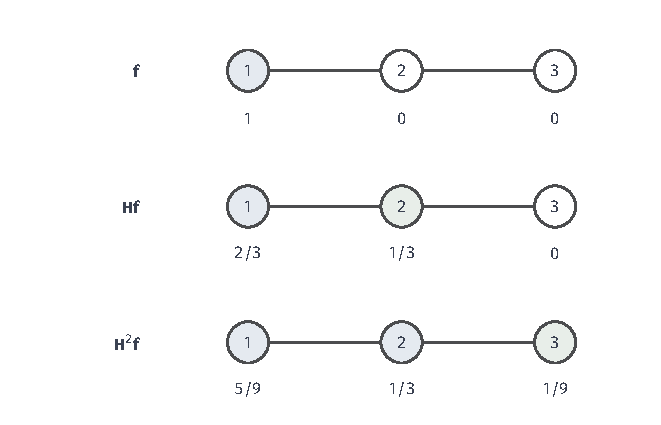
\includegraphics[width=112.0mm]{figures/00-shared/mathematical-preliminaries-upper/07-graphs/tikz/graph-theory-polynomial-locality/figure.pdf}
  \caption{三顶点路径上$H=I-L/3$的一次与二次作用：第一轮只到一跳邻居，
  二次多项式才到达两跳邻居。}
  \label{fig:graph-theory-polynomial-locality}
\end{figure}

\subsection{热扩散的谱求值法}
若每点按邻居与自身之差连续调整$f_i'(t)=\sum_j w_{i,j}(f_j-f_i)$，得到热方程
\begin{equation}
  \frac{\mathrm d\bm f(t)}{\mathrm dt}=-\bm L\bm f(t),\qquad \bm f(0)=\bm f_0,
  \label{eq:graph-theory-heat-equation}
\end{equation}
矩阵指数给出$\bm f(t)=e^{-t\bm L}\bm f_0
 =\sum_k e^{-t\lambda_k}\langle\bm u_k,\bm f_0\rangle\bm u_k$。
即取响应$g(\lambda)=e^{-t\lambda}$：零模保留、正模态按指数衰减。
\paragraph{总和守恒与分量均值}
由$\bm1^\top\bm L=\bm0$有$\frac{\mathrm d}{\mathrm dt}\bm1^\top\bm f=0$，总和守恒；
每个正权支撑分量分别趋于其初始平均（分量常方向投影为该分量平均），支撑连通时才是全图同一平均，
孤点保留自己的初值。贯穿图单位权、$\bm f_0=(1,0,0,0)^\top$、谱$0,2,4,4$，
保留比例为$1,e^{-2t},e^{-4t},e^{-4t}$，极限每点$1/4$而非归零（图~\ref{fig:graph-diffusion-spectrum}）。
\begin{figure}[htbp]
  \centering
  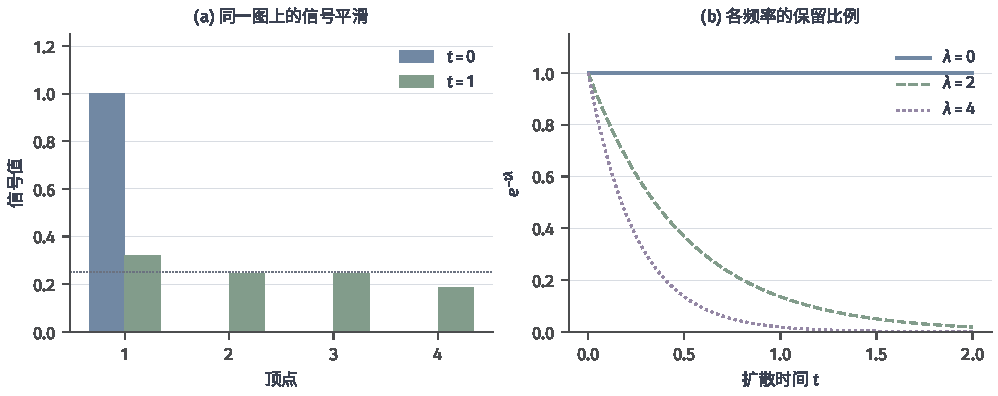
\includegraphics[width=169.0mm]{figures/00-shared/mathematical-preliminaries-upper/07-graphs/matplotlib/graph-diffusion-spectrum/figure.pdf}
  \caption{贯穿四顶点图的解析式扩散：左图比较初值$(1,0,0,0)$与$f(1)=e^{-L}f(0)$，
  灰线为极限均值$1/4$；右图示特征值$0,2,4$的保留比例（$4$重数为$2$）。}
  \label{fig:graph-diffusion-spectrum}
\end{figure}
\paragraph{两类耗散}
平方范数与边差能量是不同量：
\[
  \frac{\mathrm d}{\mathrm dt}\frac12\|\bm f\|_2^2=-\bm f^\top\bm L\bm f\leq0,\qquad
  \frac{\mathrm d}{\mathrm dt}(\bm f^\top\bm L\bm f)=-2\|\bm L\bm f\|_2^2\leq0.
\]
整体边差能量下降不保证每条边的差都单调缩小：三点路径从$(1,1,0)$出发，
边$1-2$初始差为零、其差的导数却为$1$，短时间内反而由相等变不等。
指数不是固定低阶多项式，不受有限$K$跳截断限制；时间过长会抹去分量内全部非恒定差异。

\subsection{显式Euler的局部扩散近似}
大图不便存完整谱基时，可用局部迭代近似固定时刻$T$的演化。
\begin{algorithm}[显式Euler扩散]
  选择整数$R\geq1$与步长$\tau=T/R$，令$\bm f^0=\bm f_0$，逐轮
  $\bm f^{r+1}=\bm f^r-\tau\bm L\bm f^r$（从旧向量算入独立新向量后整体替换），共$R$轮，输出$\bm f^R$近似$\bm f(T)$。
\end{algorithm}
按模态，$R$轮的系数乘子为$(1-\tau\lambda_k)^R$，而连续演化为$e^{-T\lambda_k}$；
固定$T$、$\tau\to0$（$R\tau=T$）时由$(1-x)$的一阶展开知这是时间离散近似，
误差还取决于输入在各模态上的系数，“迭代稳定”不等于“误差已足够小”。
若$d_{\max}=\max_i d_i>0$，取$R\geq\lceil T d_{\max}\rceil$可使$0<\tau\leq1/d_{\max}$、
每轮成为系数非负且和为$1$的邻居平均；要让$R\to\infty$（固定$\tau$、时间趋于无穷）时各非零模衰减，
需更严格的$0<\tau<1/d_{\max}$（用到$\lambda_{\max}(\bm L)\leq2d_{\max}$），
此时$|1-\tau\lambda_k|<1$，迭代趋于各分量均值。边界步长会失效：
单边两点图在$\tau=1$时每轮交换两端的值，系数虽仍非负却周期振荡、不收敛。
$R$轮共$O(R(n+m_+))$运算、额外$O(n)$，$R$由目标时长与精度决定，不能只报单轮成本。

\section{基于多重集合编码的1-WL标记细化法}

要知道每点周围有哪几类邻居、各出现几次，只记“出现过哪些类型”会丢次数，
按编号拼接又带入任意顺序；用\term{多重集合}同时保留种类与次数、忽略排列
（$\{\!\{a,a,b\}\!\}\neq\{\!\{a,b\}\!\}$）。

\begin{definition}[一维Weisfeiler--Leman细化]
  \label{def:graph-theory-wl-refinement}
  一维Weisfeiler--Leman细化（1-WL）从初始标记$c_i^{(0)}$出发，同步更新
  \begin{equation}
    c_i^{(t+1)}=\operatorname{HASH}\Bigl(
      c_i^{(t)},\ \{\!\{c_j^{(t)}:j\in N(i)\}\!\}\Bigr),
    \label{eq:graph-theory-wl-refinement}
  \end{equation}
  其中HASH对不同输入对给出不同新标记。
\end{definition}
HASH是无碰撞编码的数学约定，机器实现要比较完整键而非只比有限哈希值。
\begin{algorithm}[1-WL同步细化]
  本轮全部点只读旧标记，把自身旧标记与邻居标记多重集合组成的规范签名写入新数组，
  全部完成后统一替换；保存每轮分区与各类计数，直到某轮分区不再被拆分。
  比较两图时在两图不交并上共用初始标记规则与同一字典统一编码。
\end{algorithm}
三点路径初始同为$A$时，端点签名$(A,\{\!\{A\}\!\})$与中点签名$(A,\{\!\{A,A\}\!\})$不同，
第一轮分出端点类$B$与中心类$C$，下一轮签名再变但原有两类不再被拆开。
因新签名含自身旧标记，分区只能细分不能合并；每次严格细分至少多一个非空块，
故至多细分$n-1$次，一旦某轮未变以后也不会再分。
\begin{figure}[htbp]
  \centering
  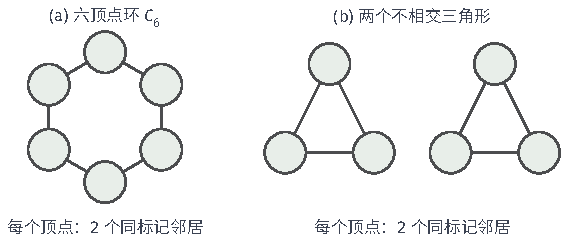
\includegraphics[width=94.936mm]{figures/00-shared/mathematical-preliminaries-upper/07-graphs/tikz/graph-theory-wl-local-ambiguity/figure.pdf}
  \caption{六环$C_6$与两个不相连三角形初始同标记，每点每轮都看到两个同类邻居，
  1-WL计数始终一致，无法区分连通的六环与两个分量。}
  \label{fig:graph-theory-wl-local-ambiguity}
\end{figure}
如图~\ref{fig:graph-theory-wl-local-ambiguity}，稳定不等于判同构：
六环$C_6$与两个不相连三角形的每点都看到两个同类邻居，计数始终一致，尽管连通分量数不同。
某轮两图计数不同可判定在当前属性设定下不同构，计数一直相同只表示本方法未区分；
给每点附唯一编号会改变所比较的问题（若属性随置换同步移动则是带属性图比较）。
等变只排除任意编号影响，既不保证完全可辨也不保证预测有效。
直接逐点排序邻居时一轮约需$O(n+m+\sum_i d_i\log(d_i+1))$加签名比较，轮数计入稳定前总时间。

\section{基于局部表汇总的配置查询方法}
\label{sec:graph-theory-semiring-dynamic-programming}

这类问题的一个顶点答案依赖所有其他变量，不能靠一次邻居加权汇总得到；
但局部因子只依赖少数变量，因此可以先消去内部变量、只把接口取值留在中间表。

\paragraph{总量、最优值与见证}
先看二元表$g=\begin{bmatrix}1&3\\2&4\end{bmatrix}$。解释为非负权重时，
总量$\sum_{x,y}g=10$，最大权重$\max_{x,y}g=4$（见证$(1,1)$）；
解释为成本时最小值$1$（见证$(0,0)$）。同一张表因查询不同输出不同。
保留$y$求和得$(3,7)$、再求和得$10$；只有当非负权重的总量$0<Z<\infty$时，
除以$Z$才得到概率，$Q(y)/Z$才是边缘概率，否则不能这样归一化；
最大化保留$y$得$(2,4)$，那是条件最优权重而非概率。

\paragraph{交换\term{半环}与分配规则}
一个配置内合并局部项记$\otimes$，跨未知变量的不同取值汇总记$\oplus$。
\begin{definition}[交换半环]
  \label{def:graph-theory-semiring}
  交换半环$(\mathcal S,\oplus,\otimes,e_\oplus,e_\otimes)$中两种运算都结合、交换并各有单位元，
  且$\otimes$对$\oplus$分配：
  \[
    a\otimes(b\oplus c)=(a\otimes b)\oplus(a\otimes c),\qquad a\otimes e_\oplus=e_\oplus.
  \]
  空汇总取$e_\oplus$，空组合取$e_\otimes$。
\end{definition}
半环不要求减法或除法。常用实例为：和积$(\mathbb R_{\geq0},+,\times,0,1)$、
最大积$(\mathbb R_{\geq0},\max,\times,0,1)$、最小加法
$(\mathbb R\cup\{+\infty\},\min,+,+\infty,0)$、布尔$(\{\mathrm F,\mathrm T\},\lor,\land,\mathrm F,\mathrm T)$。
最小加法约定$+\infty+c=+\infty$以表示不可行，对数最大加法则用$-\infty$。
没有相关因子的变量仍有状态数：和积下对$q$个状态汇总空组合$1$得到$q$，不能把该变量删掉。
局部因子按
\begin{equation}
  F(\bm z)=\bigotimes_a\phi_a(\bm z_{S_a})
  \label{eq:graph-theory-factorized-objective}
\end{equation}
组合，$S_a$是因子作用域；三元规则仍须整体保留为$\phi_{2,3,4}$，成对形式不是其等价分解。

\subsection{逐变量消元法}
\begin{algorithm}[变量消元]
  维护当前因子集合及按变量的反向索引。对消元序中每个$z_i$：收集全部含$i$的因子$\mathcal F_i$，
  其作用域并集去掉$i$得接口$R_i$；对每个接口配置枚举$z_i$，把旧因子投影取值后用$\otimes$组合、
  用$\oplus$累计，生成
  \[
    \psi_i(\bm z_{R_i})=\bigoplus_{z_i\in\mathcal Z_i}\bigotimes_{f\in\mathcal F_i}f;
  \]
  删除旧因子、以$\psi_i$替换并同步索引。保留变量不列入消元序；消到保留变量停止即得输出表，全消完得标量。
\end{algorithm}

\begin{theorem}[半环变量消除的正确性]
  \label{thm:graph-theory-semiring-elimination}
  对有限取值变量和交换半环，按任意完整次序消元所得标量等于直接枚举的全局汇总；
  保留一组输出变量时，消去其余变量所得表逐个配置等于原查询。
\end{theorem}
\begin{proof}
不变量是：固定剩余配置，当前因子的$\otimes$组合等于原函数对已消变量的$\oplus$汇总，
初始即原分解。消$z_i$时用分配律把不含$i$的因子移出汇总：
\[
  \bigoplus_{z_i}\Bigl[\bigotimes_{f\in\mathcal F_{-i}}f\ \otimes\bigotimes_{f\in\mathcal F_i}f\Bigr]
  =\Bigl(\bigotimes_{f\in\mathcal F_{-i}}f\Bigr)\otimes
   \Bigl(\bigoplus_{z_i}\bigotimes_{f\in\mathcal F_i}f\Bigr),
\]
末项即新因子$\psi_i$；结合、交换律把对$z_i$的汇总接到此前汇总之后，不变量保持，归纳即得结论。
\end{proof}
正确性对任意次序成立，但中间表代价由次序决定，这正是第~\ref{chap:graph-traversal}章诱导宽度$k_\pi$刻画的内容：
先消$1,4$接口只有$(z_2,z_3)$（二值$4$项），先消$2$则接口为$(z_1,z_3,z_4)$并产生填充边$1-4$（$8$项）。
第$i$步朴素代价约$O((b_i+1)q^{|R_i|+1})$，接口表与选择表各至多$q^{|R_i|}$项，
输出表还要另计$\prod_{i\in Q}|\mathcal Z_i|$个条目。
\paragraph{极值见证与混合汇总顺序}
最大/最小查询要为每个接口配置额外保存一个达到极值的$z_i$（选择表），
全消后取最后选择、再按消元逆序用已恢复接口值查表回溯；平局规则须事先声明，
最优值为$+\infty$表示无有限可行解。严格正权重可用负对数把最大积转成最小加法。
不同汇总一般不能换序：对$h=\begin{bmatrix}4&0\\0&4\end{bmatrix}$，
\begin{equation}
  \max_x\sum_y h(x,y)=4,\qquad \sum_y\max_x h(x,y)=8,
  \label{eq:graph-theory-max-sum-order-a}
\end{equation}
前者要求全部$y$共用一个$x$，后者允许$x$随$y$改变（图~\ref{fig:vol1-add-graph-max-sum-choice}）；
一般有$\max_x\sum_y h\leq\sum_y\max_x h$，等号需要存在对所有$y$同时最优的共同$x$。
\begin{figure}[htbp]
  \centering
  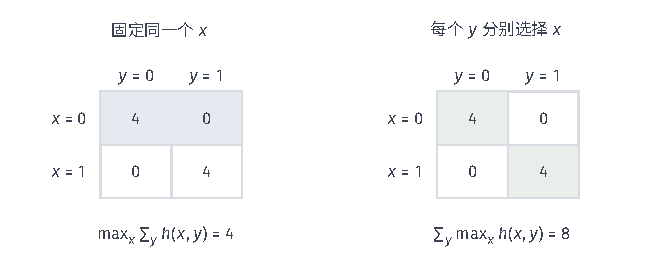
\includegraphics[width=112mm]{figures/00-shared/mathematical-preliminaries-upper/00-shared/tikz/graphs-and-signals-comprehension-additions/graph-max-sum-choice.pdf}
  \caption{同一表的两种汇总：左要求共用一个$x$（得$4$），右允许$x$随$y$变（得$8$）。}
  \label{fig:vol1-add-graph-max-sum-choice}
\end{figure}
混合求和与最大化会限制合法消元次序，所需宽度可能超过普通树宽；
连续积分换序还需Tonelli（非负）或Fubini（绝对可积）条件，不能只换符号。

\subsection{树上两遍消息传递法}
树的唯一路径使删边后的各侧子树互不重叠，可把子树概括成一张以接收变量为索引的消息。
\begin{theorem}[树消息递推]
  \label{thm:graph-theory-tree-message-recursion}
  对有限取值变量、有限树和交换半环，删边$\{u,v\}$后$u$侧子树$T_{u|v}$发给$v$的消息满足
  \begin{equation}
    m_{u\to v}(z_v)=\bigoplus_{z_u}\Bigl[
      \phi_u(z_u)\otimes\phi_{u,v}(z_u,z_v)
      \otimes\bigotimes_{r\in N(u)\setminus\{v\}}m_{r\to u}(z_u)\Bigr].
    \label{eq:graph-theory-tree-message-recursion}
  \end{equation}
\end{theorem}
对子树大小归纳即得：叶子无入消息、空组合取$e_\otimes$；非叶点删除$u$后各入向子树互不重叠、
彼此无边，归纳假设把它们概括为入消息，分配律把只依赖$z_u,z_v$的接口边移出各子树汇总。
每个顶点因子、内部边因子和接口边因子恰好计一次。
\begin{algorithm}[树上两遍消息]
  任选根，按后序从叶向根发消息并在根组合一元因子与全部入消息（再汇总根变量得总量，不汇总得根表）；
  需要每个变量的查询表时，再按前序向子节点发“排除该子树贡献”的向下消息
  （发给$v$时组合除$v$外各入消息，高度数点用前缀、后缀避免重复计算，半环无除法不能相除）。
\end{algorithm}
在路径$1-2-3$上取一元表$\phi_1=(1,3),\phi_2=(1,1),\phi_3=(2,1)$，边表同值为$2$、异值为$1$，
以$2$为根：$m_{1\to2}=(5,7)$、$m_{3\to2}=(5,4)$，根的一元因子最后乘入得根表$(25,28)$、总量$53$；
向下$m_{2\to1}=(14,13)$、$m_{2\to3}=(17,19)$，三个单点未归一化表分别为
$(14,39),(25,28),(34,19)$，各自求和都是$53$。和积下单点表还要除以同一正总量$53$，
最大/最小查询则沿向上消息另存选择并在定根后回溯。
$n$点树发$2(n-1)$条有向消息，每变量至多$q$状态时前后缀实现总量$O(nq^2)$、消息表共$O(nq)$项
（原始成对表可有$O(nq^2)$项）；只求一个根查询一次向上即可，不必机械回传。

\subsection{树分解下的袋消息法}
一般图先用第~\ref{chap:graph-traversal}章的有效树分解。把每个原因子整体归入唯一一个含其作用域的袋（只归一次），
本袋函数$\Phi_B$是这些因子的组合，无因子的袋取$e_\otimes$但仍保留变量域。
相邻袋$B,C$的接口$S_{B,C}=B\cap C$上，袋消息为
\[
  \mu_{B\to C}(\bm z_{S_{B,C}})
  =\bigoplus_{\bm z_{B\setminus S_{B,C}}}
   \Bigl[\Phi_B(\bm z_B)\otimes
     \bigotimes_{D\in N_{\mathcal T}(B)\setminus\{C\}}\mu_{D\to B}(\bm z_{D\cap B})\Bigr].
\]
运行交集保证删去一条袋树边后分居两侧的同一变量必在接口$S_{B,C}$中，
固定接口配置后两侧内部变量不重叠，才能沿用树归纳；同一变量在多个袋中是同一身份不是多个副本。
图~\ref{fig:graph-theory-bag-message-interface}中两袋$\{1,2,3\}$、$\{2,3,4\}$的接口$\{2,3\}$
有四个二值状态，左袋只汇总内部变量$z_1$发四行接口表，三元因子$\phi_{2,3,4}$完整归右袋，
接口因子只归一侧。若运行交集失效，同一变量在两枝被独立赋不同值，就不再对应任何全局配置。
\begin{figure}[htbp]
  \centering
  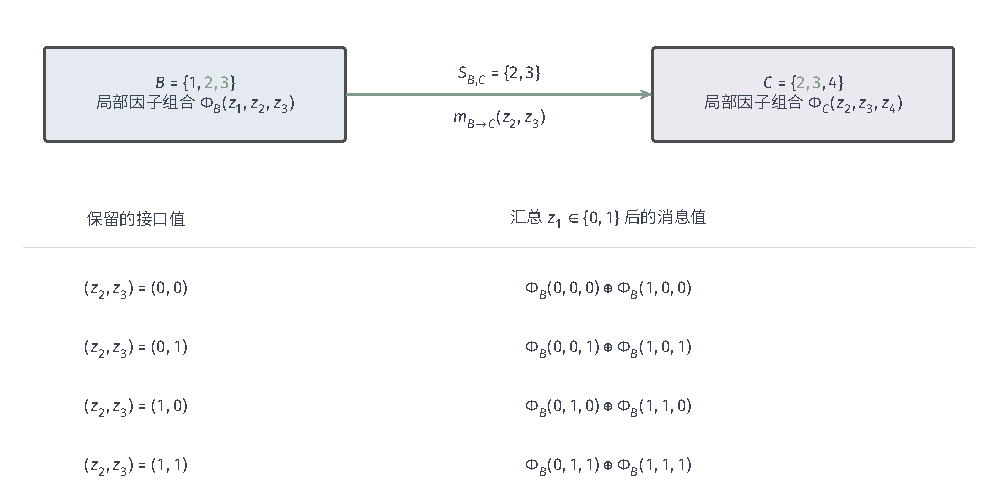
\includegraphics[width=168.998mm]{figures/00-shared/mathematical-preliminaries-upper/07-graphs/tikz/graph-theory-bag-message-interface/figure.pdf}
  \caption{两袋树分解上的叶袋消息：$B=\{1,2,3\}$只汇总内部变量$z_1$，
  经接口$\{2,3\}$向$C=\{2,3,4\}$发送四行二值接口表。}
  \label{fig:graph-theory-bag-message-interface}
\end{figure}
宽$k$、每变量至多$q$状态时每袋至多$q^{k+1}$个配置，一条袋消息需
$\prod_{i\in B\cap C}|\mathcal Z_i|$项，还要计袋数、因子读取、邻接袋数与每次运算成本；
固定$k,q$且袋数与表读取受多项式界时才有固定参数多项式保证，
寻找优分解本身另算。直接在原有环图上反复套树递推会因子树重叠而重复计数，
是否收敛、收敛到什么及误差都须另证，循环近似推断留待概率模型卷。

\section{子集格上的累计与Möbius反演}
\label{sec:comb-cumulative-inversion}

前几节的函数都定义在一张固定图的顶点或配置上。本节换一张由包含关系给出的图：
有限集合的全部子集作为顶点，只相差一个元素的两个子集之间连一条边，函数则以子集为自变量。
第~\ref{chap:counting}章的容斥原理由各交集的大小恢复并集的大小；类似的“由累计量恢复局部量”的问题也出现在一般的数值上。
设想每个课程组合有一个得分：单门课各有贡献，某两门课同时选又会产生额外的配合效果。
我们能观察到的是每个课程组合的总得分，想知道的却是每个组合自身贡献了多少。
总得分是该组合全部子组合贡献的累计，恢复自身贡献就是把这种累计倒过来。
以下$V$是有限集合，数值例子取$V_0=\{1,2,3,4\}$。

\paragraph{子集格}

累计沿包含关系进行：$S$的累计值收集所有$T\subseteq S$的贡献。
第~\ref{sec:prelim-binary-relations}节已经说明，包含关系是幂集上的偏序。
有限集合$V$的全部子集连同包含关系组成子集格：它的元素是子集，次序是$T\subseteq S$；
两个子集的交是它们最大的公共子集，并集是包含两者的最小集合。

图~\ref{fig:comb-subset-lattice-contributions}按元素个数自下而上分层画出$V_0$的子集格，
每条连线连接只相差一个元素的两个子集，沿连线向上一步就是加入一个元素。
从$S$出发沿连线一路向下能到达的子集，恰好是$S$的全部子集；
例如从$\{1,3\}$向下只能到达$\{1\}$、$\{3\}$和空集。

给每个子集$T$指定一个实数$h(T)$，表示$T$作为整体自身带来的贡献；
把$S$的全部子集的贡献相加，就得到$S$的累计值
\[
 g(S)=\sum_{T\subseteq S}h(T).
\]
$h$与$g$都是以子集为自变量的实值函数。图中的教学设定让四个单项各贡献$2$，
$\{1,3\}$另有配合贡献$3$，$\{2,4\}$另有配合贡献$-1$，其余子集的贡献为$0$。于是
\[
 g(\{1,3\})=h(\varnothing)+h(\{1\})+h(\{3\})+h(\{1,3\})=0+2+2+3=7,
\]
而两个单项的累计值之和只有$g(\{1\})+g(\{3\})=4$，多出的$3$正是$\{1,3\}$自身的贡献。
反演要回答相反方向的问题：只知道每个子集的累计值$g$，怎样读出各子集自身的贡献$h$。
\begin{figure}[htbp]
  \centering
  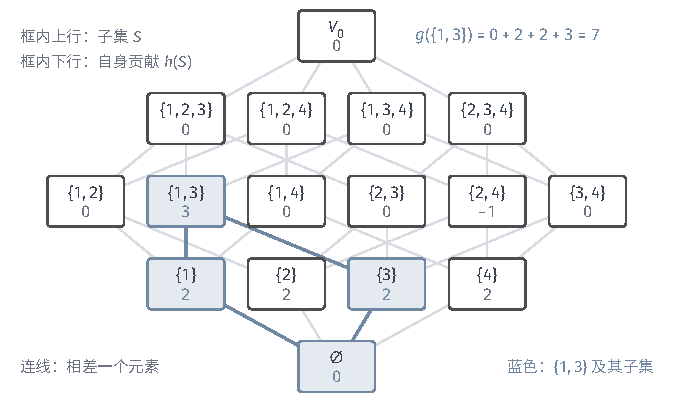
\includegraphics[width=112mm]{figures/00-shared/mathematical-preliminaries-upper/00-shared/tikz/mathematical-language-combinatorics-analysis-optimization-comprehension-additions/subset-lattice-contributions.pdf}
  \caption{四元素集合$V_0=\{1,2,3,4\}$的子集格与各子集自身的贡献。子集按元素个数自下而上分层，连线连接只相差一个元素的两个子集；每个框的上行为子集$S$，下行为教学设定的贡献$h(S)$。蓝色标出$\{1,3\}$及其全部子集，它们的贡献相加得到累计值$g(\{1,3\})=7$。}
  \label{fig:comb-subset-lattice-contributions}
\end{figure}

\paragraph{Möbius反演}

已知全部累计值$g$时，下面的\term{Möbius反演}（Möbius inversion）公式给出每个$h(S)$：
它把$S$的各子集上的累计值按元素个数之差交替加减。
\begin{theorem}[子集格上的 Möbius 反演]
\label{thm:comb-mobius-inversion}
设$V$为有限集合，$g,h:\mathcal{P}(V)\to\mathbb{R}$满足
\begin{equation}
  g(S)=\sum_{T\subseteq S}h(T)
  \qquad\text{对每个 }S\subseteq V.
  \label{eq:comb-zeta-transform}
\end{equation}
则
\begin{equation}
  h(S)
  =
  \sum_{T\subseteq S}(-1)^{|S|-|T|}g(T).
  \label{eq:comb-mobius-inversion}
\end{equation}
反过来，由式~\eqref{eq:comb-mobius-inversion}定义$h$也会恢复
式~\eqref{eq:comb-zeta-transform}。
\end{theorem}

\begin{proof}
把式~\eqref{eq:comb-zeta-transform}代入式~\eqref{eq:comb-mobius-inversion}右侧。所得双重和遍历满足$R\subseteq T\subseteq S$的全部集合对$(R,T)$；
先固定$T$与先固定$R$遍历的是同一批集合对，所以可以像第~\ref{sec:prelim-finite-sums-products}节的三角形求和那样交换有限求和的次序，得到
\begin{align*}
  \sum_{T\subseteq S}(-1)^{|S|-|T|}g(T)
  &=
  \sum_{T\subseteq S}(-1)^{|S|-|T|}
  \sum_{R\subseteq T}h(R)\\
  &=
  \sum_{R\subseteq S}h(R)
  \sum_{T:R\subseteq T\subseteq S}
  (-1)^{|S|-|T|}.
\end{align*}
固定$R$后，满足$R\subseteq T\subseteq S$的集合$T$由$S\setminus R$中哪些元素被加入决定，
即$T=R\cup D$，其中$D\subseteq S\setminus R$可以任意选取，且$|S|-|T|=|S\setminus R|-|D|$。
记$q=|S\setminus R|$，按$|D|=j$分类，大小为$j$的$D$有$\binom qj$个，所以内层和等于
\[
  \sum_{j=0}^{q}\binom{q}{j}(-1)^{q-j}
  =(-1)^q\sum_{j=0}^q(-1)^j\binom qj
  =\begin{cases}1,&q=0,\\0,&q\geq1,\end{cases}
\]
最后一步用式~\eqref{eq:comb-alternating-subset-count}。
它在$R=S$时为$1$，在$R\neq S$时为$0$，所以$S$的真子集$R$上的贡献全部抵消，只留下
$h(S)$。

反方向同样可以直接核对。由式~\eqref{eq:comb-mobius-inversion}定义$h$后，代入并交换求和次序，
\[
 \sum_{T\subseteq S}h(T)
 =\sum_{R\subseteq S}g(R)
   \sum_{T:R\subseteq T\subseteq S}(-1)^{|T|-|R|}
 =g(S).
\]
这里的内层和仍写成$T=R\cup D$，按$|D|=j$分类后等于$\sum_{j=0}^q(-1)^j\binom qj$，
它在$R=S$时只有$D=\varnothing$一项而等于$1$，在$R\neq S$时为零。
\end{proof}

\paragraph{反演的算例}

记$\mathbb I\{\text{条件}\}$在条件成立时取$1$，否则取$0$。
沿用图~\ref{fig:comb-subset-lattice-contributions}中的贡献，累计值可以直接写成
\[
 g(S)=2|S|+3\mathbb I\{\{1,3\}\subseteq S\}-\mathbb I\{\{2,4\}\subseteq S\}.
\]
其中$2|S|$收集$S$中各单项的贡献，后两项分别在$S$包含$\{1,3\}$或$\{2,4\}$时计入相应的配合贡献。
下面只用这些累计值，核对反演公式能否恢复图中的贡献；
表~\ref{tab:comb-four-element-mobius}列出全部累计值及由反演恢复的贡献。
\begin{table}[htbp]
  \centering
  \begin{tabular}{ccc@{\qquad}ccc}
    \toprule
    $S$ & $g(S)$ & $h(S)$ & $S$ & $g(S)$ & $h(S)$ \\
    \midrule
    $\varnothing$ & $0$ & $0$ & $\{1,2\}$ & $4$ & $0$ \\
    $\{1\}$ & $2$ & $2$ & $\{1,3\}$ & $7$ & $3$ \\
    $\{2\}$ & $2$ & $2$ & $\{1,4\}$ & $4$ & $0$ \\
    $\{3\}$ & $2$ & $2$ & $\{2,3\}$ & $4$ & $0$ \\
    $\{4\}$ & $2$ & $2$ & $\{2,4\}$ & $3$ & $-1$ \\
    $\{3,4\}$ & $4$ & $0$ & $\{1,2,3\}$ & $9$ & $0$ \\
    $\{1,2,4\}$ & $5$ & $0$ & $\{1,3,4\}$ & $9$ & $0$ \\
    $\{2,3,4\}$ & $5$ & $0$ & $V_0$ & $10$ & $0$ \\
    \bottomrule
  \end{tabular}
  \caption{四元素子集格上的累计值$g$与自身贡献$h$。除四个单项以及有配合贡献的
  $\{1,3\}$和$\{2,4\}$外，其余子集的自身贡献均为零。}
  \label{tab:comb-four-element-mobius}
\end{table}

例如对$S=\{1,3\}$，从$g(\{1,3\})=7$中减去两个单项的累计值，再加回空集的累计值，得到
\[
 h(\{1,3\})=7-2-2+0=3.
\]
同样，$h(\{2,4\})=3-2-2+0=-1$。对$S=\{1,2,3\}$，按子集大小分别取三元、二元、一元和空集项，
\[
 h(S)=9-(4+7+4)+(2+2+2)-0=0.
\]
图~\ref{fig:comb-mobius-cumulative-local}比较$\{1,3\}$的四个子集上的累计值与自身贡献。
\begin{figure}[htbp]
  \centering
  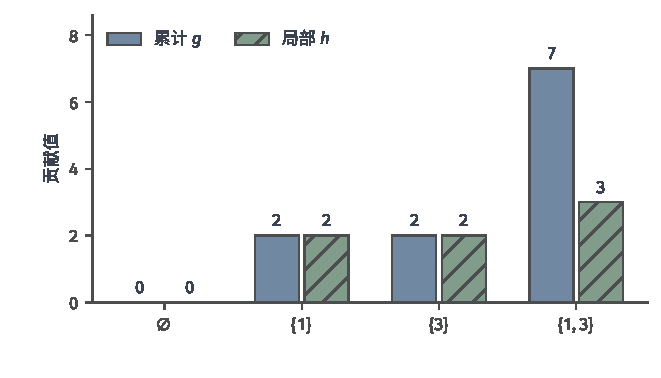
\includegraphics[width=112.0mm]{figures/00-shared/mathematical-preliminaries-upper/01-mathematical-language-combinatorics-analysis-optimization/matplotlib/comb-mobius-cumulative-local/figure.pdf}
  \caption{同一四元素教学设定在$\{1,3\}$的四个子集上的累计值与自身贡献。左侧蓝柱为$g$，右侧绿斜纹柱为$h$；
 单项贡献各为$2$，二元累计值$7$包含配合贡献$3$。四个子集的数据由正文中$g$的表达式精确计算，
 它们正是计算$h(\{1,3\})$所需的全部子集。}
 \label{fig:comb-mobius-cumulative-local}
\end{figure}

反演允许贡献取正值或负值，例如$h(\{2,4\})=-1$。它与容斥原理都依靠组合数的交错抵消，
区别在于容斥最终使并集中的每个元素恰计一次，反演最终只保留指定子集自身的贡献。

\paragraph{Möbius函数}

反演公式中的系数$(-1)^{|S|-|T|}$只依赖两个子集的相对位置。
同样的“由累计值恢复贡献”问题也可以在任意有限偏序集$(X,\preceq)$上提出，这时系数由Möbius函数给出。
记$T\prec S$表示$T\preceq S$且$T\neq S$。Möbius函数$\mu$由$\mu(S,S)=1$及
\[
 \mu(T,S)=-\sum_{T\preceq R\prec S}\mu(T,R)\qquad(T\prec S)
\]
递归定义，不满足$T\preceq S$时取$0$。
递归式的含义是：对每个$S\succ T$，从$T$到$S$之间全部系数$\mu(T,R)$（$T\preceq R\preceq S$）之和为零，这正是反演证明中内层和所需的抵消。

在子集格上，$\mu(T,S)=(-1)^{|S|-|T|}$满足这一递归：对$T\subsetneq S$，记$q=|S\setminus T|\geq1$，
则$\sum_{T\subseteq R\subseteq S}(-1)^{|R|-|T|}=\sum_{j=0}^q(-1)^j\binom qj=0$，
把$R=S$一项移到另一侧正是递归式。所以子集格上的反演系数只取$\pm1$，与定理~\ref{thm:comb-mobius-inversion}一致。

\FloatBarrier
\section{本章小结}

\paragraph{坐标变换与数值处理的区别}
谱变换把顶点值写成模态坐标，完整正反变换保持信号；按响应改变系数才是滤波。
环图可借规则FFT求值，一般图的模式由所选拉普拉斯决定。有完整谱基可直接求响应，
多项式滤波用稀疏局部更新避免求全谱，热扩散给出连续演化、Euler给出需控步长与误差的离散近似；
有限跳范围与连续扩散的全图作用不能混用。

\paragraph{数值扩散与类别细化的区别}
热扩散守恒总和、保留各正权分量的初始平均，长时间抹去分量内非恒定差异，
整体能量耗散不保证逐边单调；1-WL保留邻居类型的种类与次数并只细分不合并，
但六环与双三角形不可辨，稳定不等于同构。等变只排除编号影响，不保证可辨或预测有效。

\paragraph{配置查询的运算与接口}
配置函数评价完整赋值，局部用$\otimes$组合、跨状态用$\oplus$汇总，
能否把无关因子移出汇总取决于交换半环的分配律。消元用接口表保存内部变量贡献，
树消息与袋消息在树或有效树分解上复用这些表，精确性需要有限表、合法运算、
因子唯一归属和运行交集共同保证；见证回溯、非负归一化和混合汇总顺序各有条件。
比较方法时要同时固定图表示、函数定义域、查询输出和允许运算，再计矩阵分解、
逐轮访问、表枚举、存储与回溯——小接口或局部更新不自动使所有任务便宜，输出表本身也可能很大。

\paragraph{子集格上的累计与反演}
子集格把包含关系画成图，以子集为自变量的累计值沿向下的路径收集各子集自身的贡献；
Möbius反演按元素个数之差交替加减各子集的累计值，恢复每个子集自身的贡献，
它与容斥原理依靠同一种组合数的交错抵消，一般有限偏序上的系数由Möbius函数的递归给出。

回到章首三任务：温度平滑是数值处理，类别比较是标记细化，约束权重汇总是配置查询；
它们共享图这一组织，保存的数据和所得保证却各不相同。

\begin{table}[htbp]
  \centering\small
  \caption{本部分图方法的目标、关键条件与正确性依据。有限输入编码与数值误差仍须在实现中检查。}
  \label{tab:graph-algorithm-conditions}
  \begin{tabularx}{\linewidth}{@{}lX@{}}
    \toprule
    方法 & 关键条件与正确性依据\\
    \midrule
    Dijkstra最短路 & 边长非负；最小暂定点的归纳确定，输出距离与前驱\\
    Bellman--Ford & 允许负边；至多$n-1$边见证，可达负环后继标$-\infty$\\
    最小生成树 & 无向图、成本可负；割交换性质，输出最小连接树\\
    最大流最小割 & 非负容量、流守恒；可行流与同值割互相认证\\
    二部匹配/指派 & 二部、端点互斥；增广路径割证书，紧边势下界，指派$O(N^3)$\\
    树分解上配置查询 & 运行交集、有限状态、合法半环；指数依赖袋大小\\
    二值能量最小割 & 一元/成对成本有限且成对项次模；割容量与能量只差常数\\
    谱划分 & RatioCut/NCut只解连续松弛，取整回原目标并以下界评差距\\
    \bottomrule
  \end{tabularx}
\end{table}
